\documentclass[10pt]{article}

\usepackage[margin=1in]{geometry} 
\usepackage{amsmath,amsthm,amssymb,bbm,subcaption,graphicx,float,physics,listings,fontspec,color}
\usepackage{tikz}

\newfontfamily\Consolas{Consolas}
\definecolor{grey}{rgb}{0.9,0.9,0.9}
\lstset{basicstyle=\ttfamily, breaklines=true, numbers=left, numberstyle=\ttfamily, backgroundcolor=\color{grey}\ttfamily, keywordstyle=\color{blue}\ttfamily, stringstyle=\color{red}\ttfamily, commentstyle=\color{green}\ttfamily}
\DeclareMathOperator*{\argmin}{arg\,min}
\DeclareMathOperator*{\argmax}{arg\,max}
\DeclareMathOperator*{\Conv}{\mathop{\scalebox{1.5}{\raisebox{-0.2ex}{$\ast$}}}}
\DeclareMathOperator*{\vari}{var}

\begin{document}


% --------------------------------------------------------------
%                         Start here
% --------------------------------------------------------------
 
%\renewcommand{\qedsymbol}{\filledbox}
 
\title{\textbf{Report on Project 4}}%replace X with the appropriate number
\author{Zhunxuan Wang, 13300180086\\ %replace with your name
School of Mathematical Sciences} %if necessary, replace with your course title

\maketitle
\section{Restricted Boltzmann Machine}
\subsection{RBM Layer}
RBM is an efficient NN structure to deal with tasks regarding dimensionality reduction, classification, regression, etc. It contains a visible layer and a hidden layer, with $2$ vectors $\mathbf{b}_{\text{v}}, \mathbf{b}_{\text{h}}$ as visible bias and hidden bias, and a transition matrix $\mathbf{M}$, all of which are the parameters of the model \cite{hinton2006reducing}. The brief structure of the encoding process is shown as follows
\begin{figure}[H]
\centering
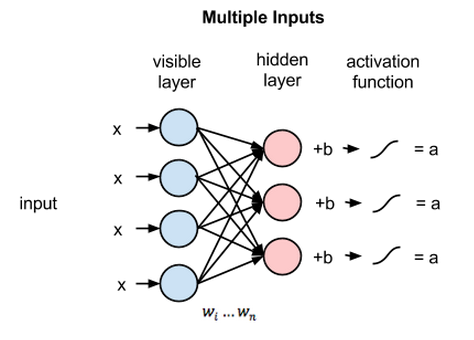
\includegraphics[scale=.5]{multiple_inputs_RBM.png}
\caption{Restricted Boltzmann Machine}
\label{rbm}
\end{figure}
The above diagram shows the encoding process from visible states to hidden states, by matrix multiplication with biases followed by activations. The formulas dominating the calculation are expressed as follows
\begin{itemize}
\item $\mathbf{x}$, $\mathbf{a}$ is the probabilities of sampling of visible state and hidden state, of which the encoding process is dominated by
$$\mathbf{a} = \sigma\left(\mathbf{x}\mathbf{W} + \mathbf{b}_{\text{h}}\right)$$
\item $\mathbf{v}$, $\mathbf{h}$ is the sampling results of visible state and hidden state, which are distributed as
$$h_i \sim \mathcal{B}\left(a_i\right)$$
where $\mathcal{B}$ is the binomial distribution.
\end{itemize}
\subsection{Reconstruction in RBM}
The reconstruction of data in RBM is based on a backward propagation in an unsupervised setting, during which the activation vector is the input and the transition weight matrix $\mathbf{W}$ remains the same (only do transpose), the bias term will be $\mathbf{b}_{\text{v}}$ which is different from $\mathbf{b}_{\text{h}}$. The backward process is shown as follows
\begin{figure}[H]
\centering
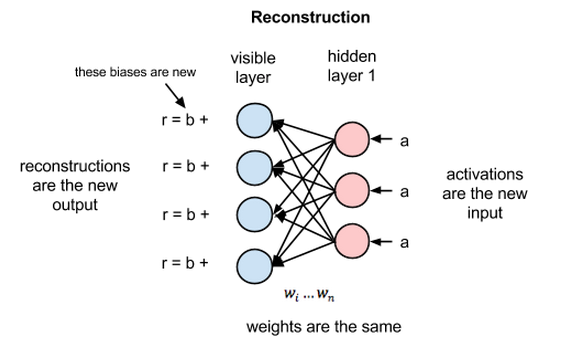
\includegraphics[scale=.6]{reconstruction_RBM.png}
\caption{Reconstruction in RBM}
\label{rec_rbm}
\end{figure}
As the diagram shows, the reconstruction process from hidden states to visible states, by matrix multiplication with biases followed by activations. The formulas dominating the calculation are expressed as follows
\begin{itemize}
\item $\mathbf{r}$ is the probabilities of sampling of reconstruction state, of which the encoding process is dominated by
$$\mathbf{r} = \sigma\left(\mathbf{a}\mathbf{W}^\intercal + \mathbf{b}_{\text{v}}\right)$$
\item The sampling is similar to the last section
$$v_i \sim \mathcal{B}\left(r_i\right)\text{.}$$
\end{itemize}
\subsection{Unsupervised Parameters Learning}
For training the $\mathbf{W}$, $\mathbf{b}_{\text{v}}$ and $\mathbf{b}_{\text{h}}$, we decide to do these on the existed model
\begin{itemize}
\item Given visible state $\mathbf{x}$, generate $\mathbf{h}$ by $\Pr\left(\mathbf{h} \mid \mathbf{x}\right)$ (the vector of sampling probabilities is $\mathbf{a}$).
\item Reconstruct to vector $\mathbf{v}$ by $\Pr\left(\mathbf{v} \mid \mathbf{h}\right)$ (the vector of sampling probabilities is $\mathbf{r}$).
\item generate hidden state again $\mathbf{h}'$ by $\Pr\left(\mathbf{h}' \mid \mathbf{v}\right)$ (the vector of sampling probabilities is $\mathbf{a}'$).
\end{itemize}
We need to make $\mathbf{x}$ and $\mathbf{v}$, $\mathbf{a}$ and $\mathbf{a}'$ closer respectively, so do the transition processes of both. Therefore the gradient of those parameters for minimizing the difference would be
\begin{align*}
\Delta\mathbf{W} &= \mathbf{x} \cdot \mathbf{a} - \mathbf{v} \cdot \mathbf{a}' \\
\Delta\mathbf{b}_{\text{v}} &= \mathbf{x} - \mathbf{v} \\
\Delta\mathbf{b}_{\text{h}} &= \mathbf{a} - \mathbf{a}'
\end{align*}
Fixing a considerable learning rate, the training would show good effects.
\section{Experimental Results}
We take the handwritten digit recognition task \texttt{MNIST} to train the RBM model. Fixing learning rate at $0.1$, and batch size $1000$, we have the following reconstruction results after $100$ iterations of training
\begin{figure}[H]
\centering
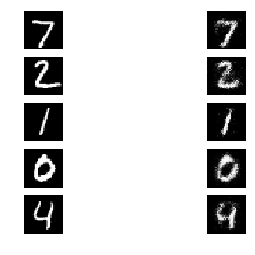
\includegraphics[scale=.7]{exp1.png}
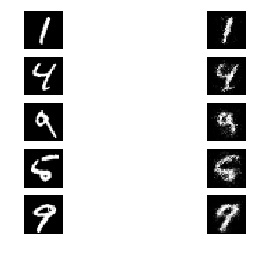
\includegraphics[scale=.7]{exp2.png}
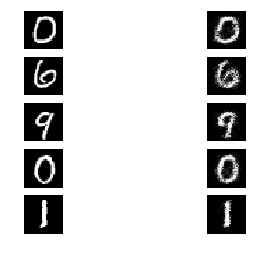
\includegraphics[scale=.7]{exp3.png}
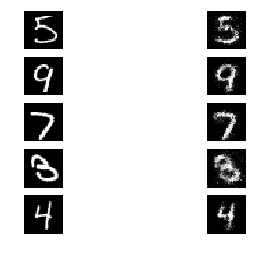
\includegraphics[scale=.7]{exp4.png}
\caption{The Reconstruction Result (original left reconstruction right)}
\end{figure}
As the results show, the shapes and contours of the image after reconstruction are basically the same as that of the originals, which means that the information (feature) extraction might be efficient. However, we can also see that the image after reconstruction becomes blurred, which means there may be loss of information.\par
We take the mean square
$$C = \frac1N\sum\limits_{i = 1}^{Nd}\norm{\mathbf{x}_i - \mathbf{r}_i}_2^2$$
as the observed cost function. The final cost is $0.0262130$.
\bigskip
\bibliographystyle{plain}
\bibliography{ref}
\end{document}